\section{チャレンジ課題2}\label{section:challenge2}
\begin{itembox}{チャレンジ課題2}
  ロジスティック回帰を実装し,
  課題1のデータに適用してテストデータの識別率を求めよ.
\end{itembox}

2クラスのロジスティック回帰モデルを実装し,課題1のデータの識別を行った.
識別率の結果は,0.875であった.

データと識別面を図に表すとを図~\ref{fig:challenge2}のようになり,識別面
がデータをクラス別に分割するように引かれていることがわかる.

\begin{figure}[htbp]
  \centering
  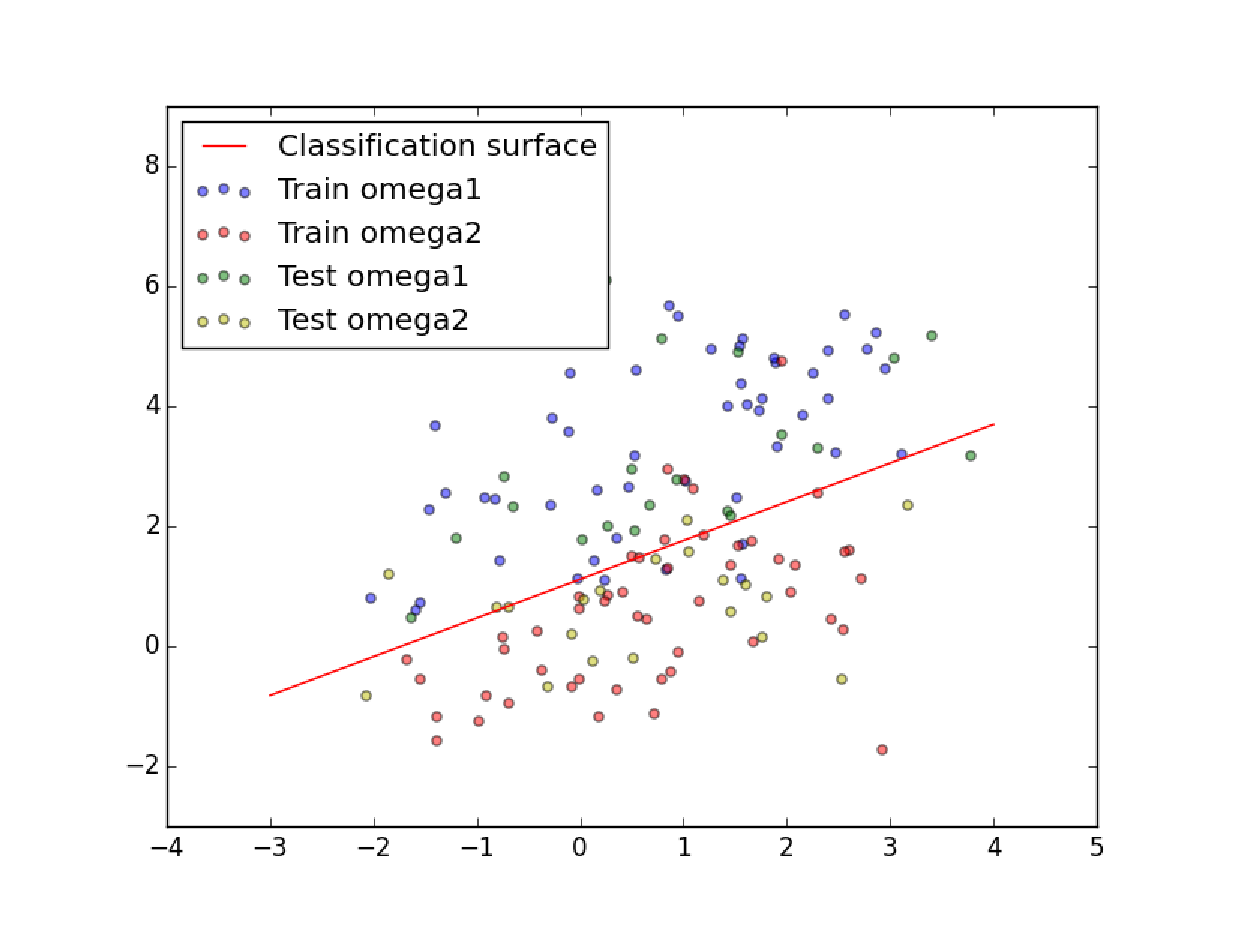
\includegraphics[width=0.8\textwidth]{./assets/challenge2_plot_20150212_000710.eps}
  \caption{ロジスティック回帰による識別}
  \label{fig:challenge2}
\end{figure}

